\documentclass[11pt]{article}

\usepackage[T1]{fontenc}
\usepackage[utf8]{inputenc}
\usepackage[a4paper,margin=1in]{geometry}
\usepackage[expansion=false]{microtype}
\usepackage{graphicx}
\usepackage{caption}
\usepackage{xcolor}
\usepackage{titlesec}
\usepackage{csquotes}
\usepackage{hyperref}

\hypersetup{
  colorlinks=true,
  linkcolor=blue!50!black,
  urlcolor=blue!50!black,
  citecolor=blue!50!black
}

% Section styling
\titleformat{\section}{\large\bfseries}{}{0pt}{}
\titlespacing*{\section}{0pt}{1.6em}{0.6em}

% Pull-quote environment
\newenvironment{pullquote}
  {\begin{quote}\itshape\color{blue!40!black}}
  {\end{quote}}


\title{\bfseries The Joy of Useless Pursuits:\\[0.3em]
       \large Why Ancient Wisdom Will Outlast AI}
\author{Souvik Sarkar \\ \texttt{sounix000@gmail.com}}
\date{July 12, 2024}

\begin{document}

\maketitle

\begin{figure}[h]
  \centering
  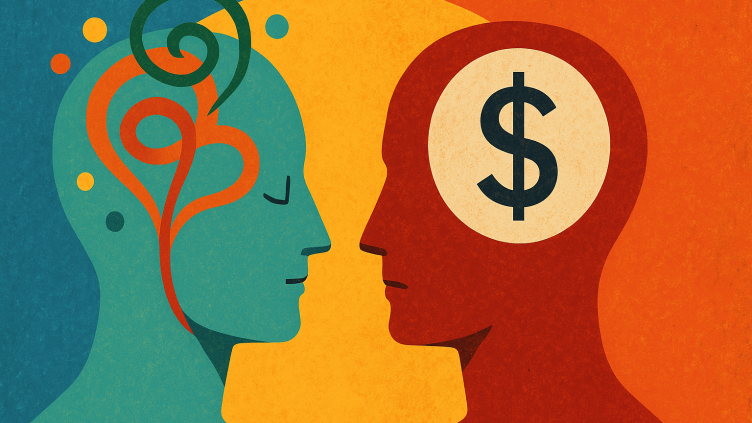
\includegraphics[width=\linewidth]{images/ai_human.png}
  \caption*{\small The irony of the fact that this image is generated by an AI, although the prompt is by the author!}
\end{figure}

There's something deeply revealing about watching a mathematician's eyes
light up when they discuss AI. While lawyers panic and consultants scramble
to prove their continued relevance, the pure theorist leans forward with
genuine excitement: \emph{Finally, a research assistant that never gets tired
of my questions!}

This split reaction tells us everything we need to know about who will thrive
when artificial minds reshape our world. The answer isn't what Silicon Valley
prophets would have us believe.

\section{The beautiful futility of pure thought}

Imagine walking through the corridors of \emph{\'Ecole Normale Sup\'erieure} in Paris, where young minds wrestle with mathematical
abstractions that have no immediate use, no clear path to profit, no obvious
benefit to humanity's material condition. These students are doing something
our productivity-obsessed age considers almost scandalous: they're thinking for
the pure joy of it.

When AI arrives to handle the world's practical problems, these
``impractical'' souls will simply continue their work, now aided by silicon
minds that can crunch numbers while leaving the deeper mysteries intact. They
were never competing with machines because they were never doing mechanical
work. They were always doing something fundamentally different:
\textbf{experiencing wonder}.

\begin{pullquote}
The crisis that's coming---and it is coming---will not be economic in the
traditional sense. It will be existential. What happens to a species that has
spent centuries defining human worth through economic utility when that utility
vanishes overnight?
\end{pullquote}

\section{The terrible honesty of obsolescence}

Every profession tells itself a story about its irreplaceable value. Lawyers
speak of nuanced judgment, consultants of strategic insight, and managers of
human leadership. But AI is offering us a terrible honesty: much of what we've
called skilled work was always pattern recognition dressed up in professional
clothing.

The panic spreading through corner offices and conference rooms isn't really
about unemployment. It's about identity collapse. These people built their
sense of self around being better than others at economically valuable tasks.
AI isn't just taking their jobs; it's revealing that their jobs were already
mechanical---the mechanism just happened to be running inside their skulls
instead of on silicon chips.

Meanwhile, in small rooms around the world, people who society has always
considered slightly mad continue their work undisturbed. The number theorist
exploring prime distributions, the poet playing with language, the philosopher
questioning the nature of consciousness---they greet our artificial future with
curiosity rather than dread because they never confused their value with their
productivity.

\section{The fraud of subsidized serenity}

We often point to Scandinavian happiness as a model for post-work society, but
this misses something crucial. Although home to serious philosophy, literature,
and math, Nordic contentment is built on oil wealth and resource extraction.
Similarly, Swiss philosophical tranquility rests on centuries of banking
profits. These societies haven't transcended economics---they've simply been
wealthy enough to afford the illusion of transcendence.

When AI disrupts the economic foundations that fund their social safety nets,
when oil becomes worthless and algorithms handle financial services, these
carefully constructed paradises may crumble faster than anyone expects. Their
happiness was always contingent, always dependent on the very economic systems
they appeared to have moved beyond.

\begin{pullquote}
True resilience lies elsewhere---in those places where intellectual fire has
burned bright even in material darkness.
\end{pullquote}

\section{The underground rivers of wisdom}

There's a reason mathematics flourished in ancient India despite economic
hardship, why poetry survived centuries of Persian upheaval, why Jewish
scholarship thrived in ghettos across Europe. These traditions understood
something we've forgotten: that the pursuit of truth and beauty needs no
external justification.

Walk into the \emph{Chennai Mathematical Institute}, where brilliant minds work with
minimal resources but maximum passion. Visit the institutes of Eastern Europe,
where scholars produced world-changing insights while their governments
collapsed around them. These are laboratories of a different kind of human
development---one that doesn't depend on venture capital or government
subsidies, but on something deeper and more durable.

\begin{pullquote}
The people in these traditions don't pursue knowledge because it might lead to
patents or profits. They pursue it because the alternative---a life without
wonder---is unimaginable.
\end{pullquote}

\section{The great returning}

What's about to happen may not be progress in the way we usually understand it,
but rather a great returning. The civilizations poised to thrive in the AI age
are not those rising now through industrial might, but those that were once
great because they understood what makes humans human.

Ancient Athens didn't fund philosophy because it generated economic growth. The
Islamic Golden Age didn't support mathematics because it improved trade
efficiency. Vedic India didn't develop complex philosophical systems to boost
agricultural output. These civilizations invested in human intellectual and
spiritual development because they recognized it as intrinsically valuable.

The industrial age convinced us to forget this wisdom. We learned to develop
human potential instrumentally---education to create workers, research to
generate competitive advantage, and even happiness policies to boost
productivity. But when AI eliminates the economic rationale for human
development, these instrumental approaches lose their foundation.

\begin{pullquote}
Societies that never lost sight of why human consciousness matters---beyond its
economic utility---will find themselves not scrambling to create meaning, but
simply continuing to pursue what they always valued.
\end{pullquote}

\section{The physics of wonder}

Here's what AI optimists and pessimists both miss: Artificial Intelligence
isn't humanity's replacement, but its liberation. Not from work---that's the
shallow reading---but from the illusion that our value lies in our usefulness.

Picture an AI tutor working with a child to rediscover the quadratic formula.
There's no rush, no economic pressure, no competition with other students. The
AI provides just enough guidance to keep the child in that magical space
between confusion and insight. When understanding finally dawns, the joy on
that child's face is purely human---the delight of a conscious mind encountering
truth for the first time.

This is what we're moving toward: a world where learning becomes play, where
research becomes art, where the ancient human love of pattern and beauty can
flourish without apologizing for its uselessness.

The civilizations ready for this transition are not those with the most
advanced technology, but those that have maintained their appreciation for what
the Greeks called \emph{theoria}---the contemplation of truth for its own sake.

\section{The deepest economics}

There's a beautiful irony waiting to unfold. The countries that prioritize
happiness, health, and intellectual contribution for their own sake---rather
than as inputs to economic output---may find themselves not just spiritually
richer, but materially more resilient as well.

\begin{pullquote}
These three elements form the true foundation of any economy: flourishing
consciousness, vital bodies, creative minds. We've spent centuries treating them
as byproducts of economic activity, when in fact they are its source.
\end{pullquote}

When the age of artificial intelligence fully arrives, the societies that
remember this truth will discover something remarkable: they were preparing for
the future all along, not by racing toward it, but by preserving what was always
most valuable about being human.

The future belongs not to those who can compete with machines, but to those who
remember why consciousness itself is worth celebrating. In our rush toward
artificial minds, the deepest victory may belong to those who never forgot the
irreplaceable miracle of the natural ones we already possess.

\begin{pullquote}
As humans, the return to useless pursuits might be our only true superpower.
\end{pullquote}

\end{document}
